\documentclass[tikz]{standalone}
\usepackage{fourier}
\usepackage{tikz}

\begin{document}
	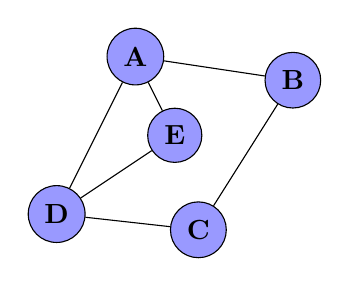
\begin{tikzpicture}
		\node[draw,circle,fill=blue!40!white](a) at (1,2) {\textbf{A}};
		\node[draw,circle,fill=blue!40!white](b) at (3,1.7) {\textbf{B}};
		\node[draw,circle,fill=blue!40!white](c) at (1.8,-0.2) {\textbf{C}};
		\node[draw,circle,fill=blue!40!white](d) at (0,0) {\textbf{D}};
		\node[draw,circle,fill=blue!40!white](e) at (1.5,1) {\textbf{E}};
		\draw (a)--(b) (b)--(c) (c)--(d) (d)--(e) (e)--(a) (d)--(a);
	\end{tikzpicture}
\end{document}
